\documentclass{article}
\usepackage[utf8]{inputenc}
\usepackage{algorithm}
\usepackage{algorithmic}
\usepackage{fancyhdr}
\usepackage{graphicx}
\usepackage[
    backend=biber, 
    natbib=true,
    style=numeric,
    sorting=none
]{biblatex}
\addbibresource{reference.bib}
\usepackage{listings}
\usepackage{xcolor}
\graphicspath{ {./images/} }

%New colors defined below
\definecolor{codegreen}{rgb}{0,0.6,0}
\definecolor{codegray}{rgb}{0.5,0.5,0.5}
\definecolor{codepurple}{rgb}{0.58,0,0.82}
\definecolor{backcolour}{rgb}{0.95,0.95,0.92}

%Code listing style named "mystyle"
\lstdefinestyle{mystyle}{
  backgroundcolor=\color{backcolour},   commentstyle=\color{codegreen},
  keywordstyle=\color{magenta},
  numberstyle=\tiny\color{codegray},
  stringstyle=\color{codepurple},
  basicstyle=\ttfamily\footnotesize,
  breakatwhitespace=false,         
  breaklines=true,                 
  captionpos=b,                    
  keepspaces=true,                 
  numbers=left,                    
  numbersep=5pt,                  
  showspaces=false,                
  showstringspaces=false,
  showtabs=false,                  
  tabsize=2
}

%"mystyle" code listing set
\lstset{style=mystyle}

\pagestyle{fancy}
\fancyhf{}
\rhead{Computer Graphics}
\lhead{CS 440}
\cfoot{\thepage}

\begin{titlepage}
    \begin{center}
        \vspace*{1cm}
            
        \Huge
        \textbf{Unraveling Syntheses of Sight and Sound}
            
        \vspace{0.5cm}
        \LARGE
        Final Project for \\
        CS 440 - Computer Graphics - L1
            
        \vspace{1.5cm}
            
        \textbf{Syed Ammar Mahdi (03691) \\ Fatima Nadeem (03768) \\ Kabir (03925)}
            
        \vfill
            
        A thesis presented for the degree of\\
        Doctor of Philosophy
            
        \vspace{0.8cm}
            
            
        \Large
        Department Name\\
        University Name\\
        Country\\
        Date
            
    \end{center}
\end{titlepage}

\begin{document}

\tableofcontents
\newpage
\section{Abstract}

The interplay between music and images lends itself to interesting approaches in a computer graphics context. A musical piece can have multiple subjective visual representations, but finding a mapping from sound to image that allows the viewer to infer some musical properties of the music is a daunting task. In this paper we discuss a novel approach to mapping a chord progression in a piece of music to different colours, using some of the techniques that were discussed in CS-440 (namely interpolation). The approach outlined here maps all 12 notes of the western chromatic scale to the 12 colours of the RGB colour wheel, then bases. The output is a grid of pixels where each chord is represented as a line of interpolated pixels; this attempts to visually represent the melodic and subjective emotional content of different chords to colours in an image. For the implementation, the myimage class in python was used, which was introduced in the first assignment.

\section{Introduction}

The primary concern of Computer Graphics is to 'display pretty pictures on a computer'\footnote{Saleem, Waqar. "CS 440: Lecture 1." Habib University, August. 2020}. Similarly, music is a way of arranginig aesthetically pleasing sounds together in a wa



Light and sound are both natural phenomenon that occur within the universe as waves; light being a transverse wave, and sound being a longitudinal wave. It is not the physics of these wave phenomenon that is of primary interest to the computer scientist, however, as much as how they can be modelled on a computer. To understand how light and sound can be modelled in meaningful ways on a computer, it is first important to understand how human beings perceive these natural phenomenon.

A sound wave can 
Human hearing is similar to light in the sense that sounds and light are both logarithmic. The human eye corresponds to changes in brightness on the visible light spectrum in a similar way to how the ear perceives sounds on the decibel scale; each subsequent increase is loudness or brightness is not perceived as a linear increase, but a logarithmic one. Both light and sound are waves that are picked up by human sensory organs and correspond to a phenomenon in the brain. Just as vision in computer graphics is modelled based on the human eye and visual system (as we saw in the first module of the course), so too can sound be modelled based on the human hearing system and how the brain perceives pitches.

Keeping these similarities between the phenomenon of vision and hearing in mind, one can then consider what qualities of vision and sound must be captured in a model to convert between the two. To do so one needs a mapping matrix, as shown in the image above. For our research we will consider a simplified mapping matrix that will consider timbre and pitch in the sound domain and map it in the image space of brightness and colour.

The question of converting between sound and colour and vice versa is not a trivial one; it can have important applications for conveying information to those deprived of one sense or the other. For example, we can consider how a blind human who cannot see any images would instead interpret a meaningful sound representation of the same image. Similarity, a deaf individual attending an electronic music festival might not be able to see hear the music being played, but can interpret the visuals being displayed as the music plays to have an aesthetic experience; after all, colour has been shown to psychologically affect the mood of a human just as listening to a piece of music can invoke strong emotions in a person.

\section{Literature Review}
This section is dedicated to discussing the different research works that were researched as part of this project. Firstly, the main paper that guided our implementation as well as provided the impetus for it is discussed. Following that, the section goes into other helpful and related works.

\subsection{Main Work Regardng Image to Sound Coversion}
The paper in question here is \cite{margounakis2006converting}. The paper basically dives into the problem by providing a mapping between image and sound characteristics. It uses this mapping to launch some concepts such as chromatic bricks and segments that make up a particular image while also specifying the notes for a melodic composition as well. The paper and its methodology served as a direct inspiration for the one developed for this project and focused on aspects it discussed, e.g. the smooth transitioning of color


\section{Our Method}

Our approach is a novel one in colour representations of a musical piece. The basic idea is to take the chord progression in a piece of music, find out the notes in the relevant chord and the colour each note is mapped to, then interpolate between the colours of the chord/notes. This will then display a line of interpolated pixels in the output pixel grid image. The details of this method are elucidated in the sections below.

\subsection{Theory}

The basic c

\subsubsection{The Mapping}

In the western musical systems, there are musical notes; these notes are collectively referred to what is known as the chromatic scale. The notes in the chromatic scales are as follows:

\begin{center}
    {A, A\#/Bb, B, C, C\#/Db, D, D\#/Eb, E, F, F\#/Gb, G, G\#/Ab}
\end{center}

This can be much more easily visualized using the keys on a piano as detailed in the figure\footnote{source: https://www.piano-keyboard-guide.com/wp-content/uploads/2015/04/piano-chromatic-scale.jpg} below:

\begin{figure}
    \centering
    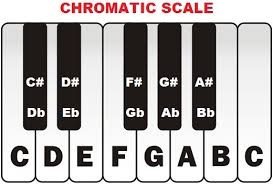
\includegraphics{chromatic.jpg}
    \caption{The western chromatic scale.}
    \label{fig:chroma}
\end{figure}

The X\#/Yb notes above (where {X, Y} represent any of the musical notes) are what are known as 'accidentals', or the black keys on the piano. Here we will use the 'sharp' (X\#) representation of an accidental, for simplicity's sake.\\

The chromatic scale has a modular structure; that means that the note C will be the next note after G\#, just an octave above the previous C note.\\

The RGB colour wheel in its most common representation has 12 colours, as detailed in the figure\footnote{source: https://i.pinimg.com/originals/ad/4b/cf/ad4bcfcd6b94b8be1aaa9717c08ff580.png} below:

\begin{figure}
    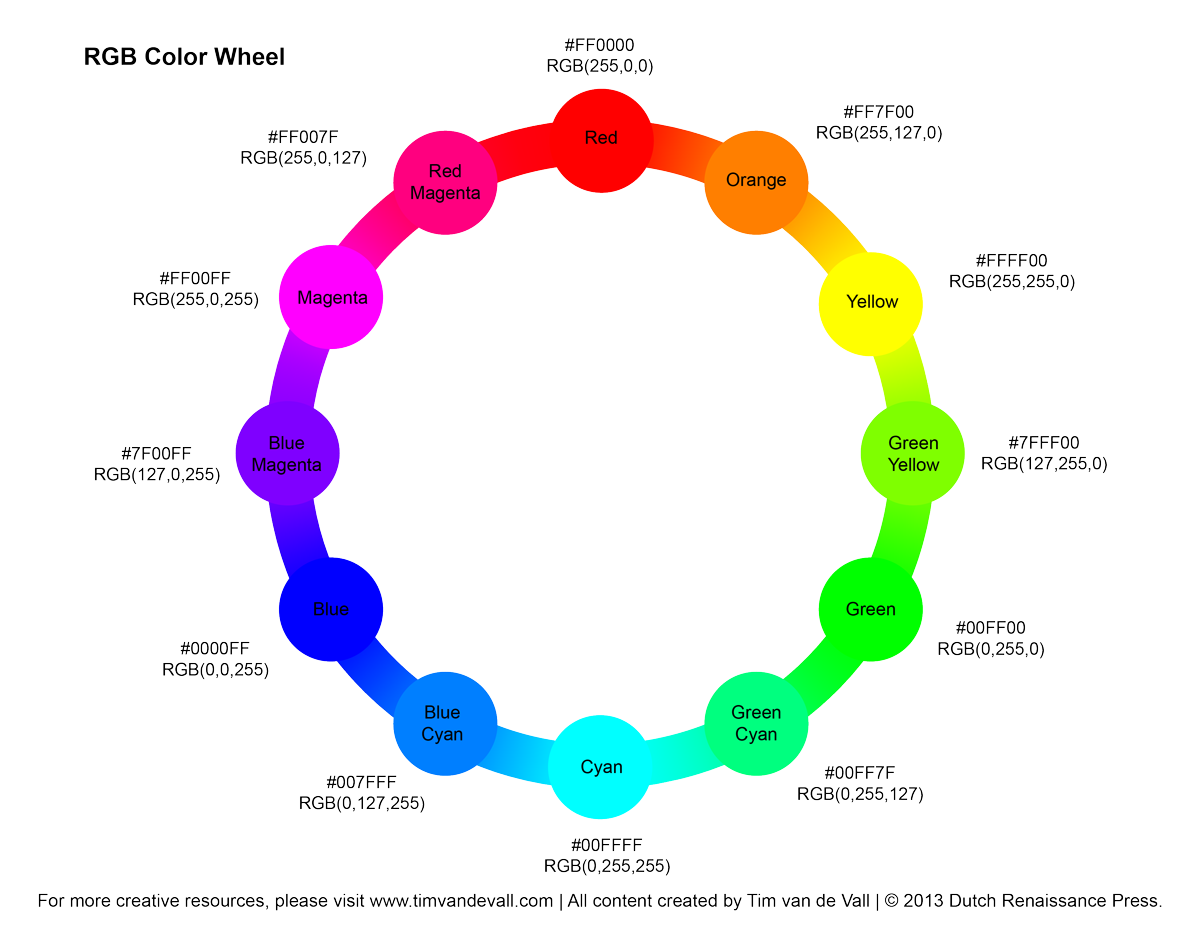
\includegraphics[scale=0.3]{wheel.png}
    \caption{A commonly used representation of the RGB colour wheel with its respective RGB values.}
    \label{fig:wheel}
    \centering
\end{figure}

One can then imagine a simple mapping between the 12 notes in the chromatic scale and the 12 colours on the colour wheel. Using this as our starting point, we can move on to colour representation of chords from the mapping defined above, which will then interpolate the colours in the chord depending on the notes.

% Required music theory definitions 
% How does the final image represent music - timewise and musicwise (This could have further sections)
\subsection{Resources}
% Python as the code coding language
% Github for collaboration
% Individual libraries and their purposes
\section{Code}
\section{Input \& Output}
% will include one or more examples of musical source and the corresponding generated image
\section{Conclusion}

\printbibliography

\end{document}
